\documentclass[a4paper,notitlepage,11pt]{article}

\usepackage[ansinew]{inputenc}
%\usepackage[frenchb]{babel}
\usepackage{graphicx} 
\usepackage[lmargin=2.0cm, rmargin=2.0cm,bottom=2.55cm,top=2.4cm]{geometry} 
\usepackage{amsmath}
\usepackage{amsthm} 
\usepackage{amssymb}  
\usepackage{eurosym} 
\usepackage{enumitem} 
\usepackage{url}
%\usepackage{bbold}
\usepackage{psfrag}
\usepackage{tikz}

\newcommand{\X}{X}
\newcommand{\Y}{Y}

\begin{document}

\setlength{\parindent}{0pt}
\setlength{\parskip}{1ex plus 0.5ex minus 0.2ex}

\Large

\textbf{Session 11:  Coalitions}

%\section*{Exercices}


%\newpage

\paragraph{1. } Alice, Bob and Carol wish to connect to the Internet. The cost of such a connection depends on the total length of cables that it requires. Of course, the players also need to be connected to the provider $\Omega$. The costs of the possible connections are given by the following graph.
\begin{figure}[!ht]
	\begin{center}
		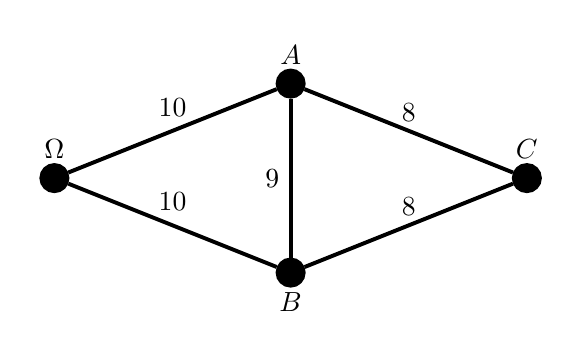
\begin{tikzpicture}[scale=2,looseness=.8,auto]
			\begin{scope}[every node/.style={font=\small\itshape},line width=0.5mm]
				\tikzstyle{every node}=[draw,fill=black,shape=circle,line width=0.5mm,minimum size=1.5mm,label distance=1mm];
				\path (0  , 0  ) node (v0) {} node [above,draw=none,fill=none] {$\Omega$};
				\path (1.5,  .6) node (vA) {} node [above,draw=none,fill=none] {$A$};
				\path (1.5, -.6) node (vB) {} node [below,draw=none,fill=none] {$B$};
				\path (3  , 0  ) node (vC) {} node [above,draw=none,fill=none] {$C$};
				\draw (v0) -- (vA) node [midway,above,draw=none,fill=none,yshift=-1mm] {$10$};
				\draw (v0) -- (vB) node [midway,above,draw=none,fill=none,yshift=-1mm] {$10$};
				\draw (vA) -- (vB) node [midway,left,draw=none,fill=none,xshift=1mm] {$9$};
				\draw (vA) -- (vC) node [midway,above,draw=none,fill=none,yshift=-1mm] {$8$};
				\draw (vB) -- (vC) node [midway,above,draw=none,fill=none,yshift=-1mm] {$8$};
			\end{scope}
		\end{tikzpicture}
	\end{center}
\end{figure}

Therefore, connecting all the players has a total cost of 26, an amount that they then need to share. Furthermore, for each player, being connected to the Internet represents a profit of 20.
\begin{enumerate}
	\item[a.] If the players can agree on a division of connection fees, what solution do you propose?
%	what is the \emph{core} in which they will choose their individual costs?
	\item[b.] Suppose you were the provider, and that you wanted to impose costs that are as honest as possible. How would you divide the costs?
\end{enumerate}

\paragraph{2. } An owner wishes to hire staff to grow potatoes in his field. If $k$ people work the land (including the owner), they produce potatoes for a value of $f(k)$. Suppose that the function $f$ is increasing, that $f(0) = 0$ and that the contribution of an additional person strictly decreases (that is to say, $f(k) - f(k-1)$ is strictly decreasing). The aim is for stakeholders to negotiate their wages. Let $n$ be the number of people working the land, and $x_i$ be worker $i$'s salary, with $x_1$ being the salary of the owner. We know that $x_1 + \dots + x_n \leq f(n)$.
\begin{enumerate}
	\item[a.] Can a worker claim a wage $x_i > f(n) - f(n-1)$? What would happen then? (Hint: describe the core of the game).
	\item[b.] Now suppose that all workers agree that none of them should engage unless it is as a group. What happens to the core in this case?
	\item[d.] Suppose now that $f(k) - f(k-1)$ is strictly increasing. Show that the core of this game contains the uniform vector of wages, that is, where each player receives an equal share of the produced wealth. (Hint: Since $f(k) - f(k-1)$ is increasing, we can show that  $\frac{f(k)}{k} < \frac{f(k + 1)}{k + 1} $ for all $k$, and $f(n)/n \leq (f(n) - f(k))/(n-k)$. )
\end{enumerate}
	


\section*{Reminders}

\begin{itemize}[leftmargin=*]
\renewcommand{\labelitemi}{$\bullet$}

	
	\item \textbf{The notion of core}
	\vspace{.3cm}

	Let $N$ be the grand coalition of all players and $v$ be the characteristic function that associates a value $v (S)$ to any coalition $S \subseteq N$. An allocation of payoffs $x$ is the \emph{core} of $v$ iff
	\begin{align*}
		\sum_{i \in N}{x_i} = v(N) \text{ et } \sum_{i\in S}{x_i} \geq v(S), \quad \forall S \subseteq N
	\end{align*} 
	where the second condition requires that no coalition can improve the payoffs of its participants.

	\vspace{.3cm}
	\item \textbf{The Shapley value}
	\vspace{.3cm}
	
	The Shapley value if the only function $\phi$ that satisfies the following behavioral axioms:
	\begin{enumerate}
		\item \textbf{Symmetry}: If one permutes the order of the players and that Player $i$ becomes Player $j$, then the Shapley value for Player $i$ in the original game has to be equal to that of Player $j$ in the new game.
		\item \textbf{Support}: If a player has nothing to bring to the coalition, he earns nothing.
		\item \textbf{Linearity}: For all characteristic function $v$ and $w$, for all $0 \leq p \leq 1$ and for all player $i$: $\phi_i(pv + (1-p)w) = p\phi_i(v) + (1-p)\phi_i(w)$.
	\end{enumerate}
	These a priori reasonable axioms lead to a unique solution, including situations in which the core is empty. The Shapley values can be explicitly computed by:
	\begin{align*}
		\phi_i(v) = \sum_{S \subseteq N -i}{\dfrac{|S|!(|N| - |S| - 1)!}{|N|!} (v(S \cup {i}) - v(S))}.
	\end{align*}
	
\end{itemize}

\end{document}










